% Project:     IMP project
% @file        doc/documentation.tex
% @date        12.12.2023
% 
% @brief Simulation study file
%
% @author Adam Ližičiar <xlizic00@stud.fit.vutbr.cz>

\documentclass[a4paper, 11pt]{article}

\usepackage[slovak]{babel}
\usepackage[utf8]{inputenc}
\usepackage[left=2cm, top=3cm, text={17cm, 24cm}]{geometry}
\usepackage{times}
\usepackage{verbatim}
\usepackage{enumitem}
\usepackage[slovak, boxed]{algorithm2e}
\usepackage{listings}
\usepackage{color}
\usepackage{graphicx}
\usepackage{tabularx}
\usepackage[unicode]{hyperref}
\hypersetup{
    colorlinks=true,
    linkcolor=black,
    urlcolor=blue, 
    citecolor=blue
}
\definecolor{mygreen}{rgb}{0,0.6,0}
\definecolor{mygray}{rgb}{0.5,0.5,0.5}
\definecolor{mymauve}{rgb}{0.58,0,0.82}
\lstset{
  backgroundcolor=\color{white},
  basicstyle=\footnotesize,
  breaklines=true,
  captionpos=b,
  commentstyle=\color{mygreen},
  escapeinside={\%*}{*)},
  keywordstyle=\color{blue},
  stringstyle=\color{mymauve},
  tabsize=4
}


\begin{document}

	%%%%% Titulná stránka %%%%%
	\begin{titlepage}
		\begin{center}
			
\includegraphics[width=0.77\linewidth]{resources/logo_FIT.pdf} \\

			\vspace{\stretch{0.382}}

			\scalebox{2}{Meranie vzdialenosti ultrazvukovým senzorom} \\
			\LARGE{Mikroprocesorové a vestavěné systémy, FIT VUT} \\
			\vspace{\stretch{0.618}}
		\end{center}

		\begin{minipage}[b]{0.4 \textwidth}
			\raggedright
			{\Large \today}
		\end{minipage}
		\hfill
		\begin{minipage}[b]{0.6 \textwidth}
			\raggedleft
			\Large
			Adam Ližičiar (xlizic00)\\
		\end{minipage}		
	\end{titlepage}

	%%%%% Obsah %%%%%
	\pagenumbering{roman}
	\setcounter{page}{1}
	\tableofcontents
	\clearpage

	\pagenumbering{arabic}
	\setcounter{page}{1}
	
	%%%%% Úvod %%%%%
	\section{Úvod}
	Táto dokumentácia opisuje spôsob zapojenia a~implementácie ultrazvukového merača vzdialenosti HY-SRF05 spolu s~segmentovým LED displejom na~vývojovej doske FITkit3.

    %%%%% Komponenty %%%%%
	\section{Komponenty}
    
	\subsection{Vývojová doska}
    Ako vývojová doska je~použitá platforma FITkit. Je to samostatné zariadenie, ktoré obsahuje výkonný mikrokontrolér s~nízkou spotrebou, hradlové pole FPGA
    (Field Programmable Gate Array) a~množstvo periférií. Dôležitým aspektom je~využitie pokročilého reprogramovateľného hardvéru na~báze hradlových polí FPGA,
    ktorý je~možné, podobne ako softvér na~počítači, neobmedzene modifikovať pre~rôzne účely podľa potreby - takže používateľ nemusí vytvárať nový hardvér
    pre~každú aplikáciu znovu.\cite{FITkit}\newline
    
    \subsection{Ultrazvukový merač vzdialenosti}
    Ultrazvukový senzor SRF05 je~zariadenie využívané na~meranie vzdialenosti pomocou vysielania a~prijímania ultrazvukových signálov. Jeho minimálny dosah
    je~približne 9~centimetrov, pričom maximálny dosah sa~pohybuje okolo 2~metrov v~závislosti od~podmienok prostredia a~presnosti merania.\cite{SRF05}

    \subsection{Segmentový LED displej}
    Na~segmentovom LED displeji je~každý segment malá LED dióda, ktorá môže byť zapnutá alebo vypnutá na~zobrazenie určitého znaku.
    Tieto segmenty sú~často organizované do matice, pričom každý segment reprezentuje číslicu alebo znak.
    Segmentový displej pozostáva zo~štyroch segmentov, ktoré sú usporiadané tak, aby~vytvorili číslice od~0 do~9. 

    %%%%% Implementácia %%%%%
    \section{Implementácia}
    Chod celého zariadenia riadi funkcia \texttt{main()}. Na začiatku sú najskôr inicializované všetky potrebné veci a následne
    sa cyklicky odosiela ultrazvukovému meraču vzdialenosti signál. Po odoslaní začne bežať časovač až do príchodu spätného signálu z merača
    vzdialenosti. Následne je toto číslo podla rovnice prevedené na vzdialenosť v centimetroch.
    \begin{lstlisting}[language=C, caption={Funkcia main()}]
/*
 * 	Main function
 */
int main(void) {

	Init(0x200);

    while (1) {

		// Reset variables
		sensorMeasuresDistance = 1;
		senzorDistance = 0;

    	// Send signal
    	PTA->PDOR |= PIN_SEND;
    	delay(50);
    	PTA->PDOR &= ~PIN_SEND;

		// Receive signal
		while (sensorMeasuresDistance)
			senzorDistance++;

		// Transform sensor response to centimeters
		distance = (senzorDistance * 0.36) / 58;


		delay(500000);

    }

    return 0;

}
    \end{lstlisting}

    \subsection{Meranie vzdialenosti}
    Pre meranie vzdialenosti je najskôr potrebné odoslať na vstup senzora Trig signál a potom čítať vrátený signál z výstupu senzora Echo.
    Následne sa vzdialenosť vypočíta podľa vzorca \texttt{distance = (senzorDistance * 0.36) / 58}.\cite{SRF05}

    \begin{figure}[!ht]
		\centering
		\vspace{1cm}
		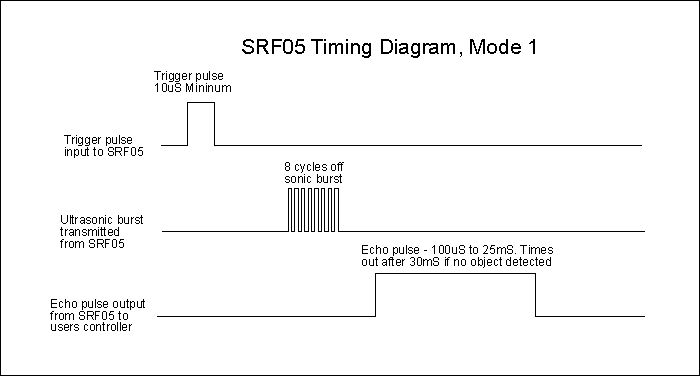
\includegraphics[width=0.95\linewidth]{resources/sensor_srf05.png}
		\caption{Meranie vzdialenosti ultrazvukovým meračom vzdialenosti SRF05\cite{SRF05}}
		\label{figure:finalStateMachine}
	\end{figure}

    \subsection{Výpis na displej}
    Písanie čísel na LED displeji je riadené elektronickým obvodom, ktorý spína jednotlivé segmenty LED v závislosti od funckie \texttt{void writeDigitOnDisplay(int number)} .
    Každé číslo sa zobrazuje zahájením a vypnutím rôznych segmentov LED, ktoré sú v určitom vzore zoskupené na displeji. Funkcia
    \texttt{activateDigit()} ovláda jednotlivé segmenty v reakcii na parameter tejto funckie.

    \begin{figure}[!ht]
		\centering
		\vspace{1cm}
		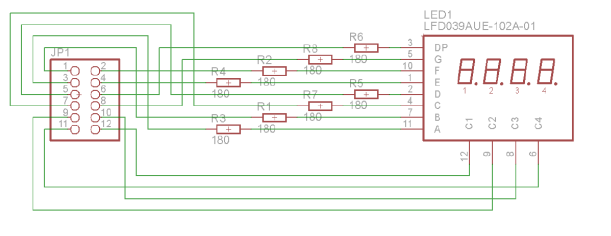
\includegraphics[width=0.95\linewidth]{resources/displej_schema_zapojenia.png}
		\caption{Schéma zapojení modulu s LED displejem\cite[snímka 4]{PresentationForProject}}
		\label{figure:finalStateMachine}
	\end{figure}


    \section{Demonštrácia fungovania}
    Ukážka funkčnosti je umiestnená na linku \href{https://youtu.be/G8GsflSrfUI}{https://youtu.be/G8GsflSrfUI}

    %%%%% Záver %%%%%
	\section{Záver}
	Program funguje správne okrem hodnôt pod 9 cm a nad približne 40 cm. Dôvodom tejto vlastnosti sú schopnosti ultrazvukového merača diaľky
    merať vzdialenosť iba na určitú dĺžku. Žiadne iné problémy sa pri tvorbe projektu nevyskytli.

 
	%%%%% Literatúra %%%%%
    \newpage
	\section{Literatúra}
	\bibliographystyle{bibliography/czechiso}
    \renewcommand{\refname}{}
	\bibliography{bibliography/documentation}

\end{document}
